% From mitthesis package
% Version: 1.07, 2024/09/26
% Documentation: https://ctan.org/pkg/mitthesis


\chapter{Quantum Arithmetic Circuit Design for Double-Factorized Electronic Structure Hamiltonian Simulation}

We now propose and analyze a quantum circuit that approximately simulates $U_A^{(r)}$ from \eqref{eq: expansion}.

\begin{equation}
    U_A^{(r)} = e^{-\frac{i\Delta t}{2}\lambda_r\left(\sum_s \lambda'^{(r)}_s n_s\right)^2} \label{eq: U_A}
\end{equation}

We can substitute the number operator correspondance from \eqref{eq: JWnum} to find the equivalent qubit operator.

\begin{equation}
    U_A^{(r)} = e^{-\frac{i\Delta t}{2}\lambda_r\left(\sum_s \lambda'^{(r)}_s n_s\right)^2} \leftrightarrow e^{-\frac{i\Delta t}{2}\lambda_r\left(\sum_s \lambda'^{(r)}_s \ket{1}\bra{1}_s\right)^2}
\end{equation}

This qubit operator, when acting on a qubit computational basis state $\ket{\vec{x}}$, simply applies a phase shift that is a function of $\vec{x}$.

\begin{equation}
    e^{-\frac{i\Delta t}{2}\lambda_r\left(\sum_s \lambda'^{(r)}_s \ket{1}\bra{1}_s\right)^2}\ket{\vec{x}} = e^{-\frac{i\Delta t}{2}\lambda_r\left(\sum_s \lambda'^{(r)}_s x_s\right)^2}\ket{\vec{x}}
\end{equation}

We want to find an efficient way to approximately simulate $U_A^{(r)}$. That is, we want to find an operator $\tilde{U}_A^{(r)}$ that applies the specified phase rotation on $\ket{\vec{x}}$ as precisely as possible and with as few gates as possible. As a reminder, the error (and therefore precision) is measured by the operator norm of the difference in the ideal and approximate operators. The parameter $\epsilon$ limits the maximum error of this approximation and it affects the cost of $\tilde{U}_A^{(r)}$. A tighter bound requires more gates to achieve that bound.

\begin{equation}
    \epsilon \geq ||U_A^{(r)} - \tilde{U}_A^{(r)}|| = ||e^{-\frac{i\Delta t}{2}\lambda_r\left(\sum_s \lambda'^{(r)}_s \ket{1}\bra{1}_s\right)^2} - \tilde{U}_A^{(r)}|| \label{eq: error}
\end{equation}

The expansion method in \eqref{eq: expansion} simulates but requires $O(n^2)$ non-Clifford gates, leading to a $O(n^2\log_2{\frac{n}{\epsilon}})$ $T$-count. We now present a $\tilde{U}_A^{(r)}$ that requires $O(n\log_2(\frac{n}{\epsilon}) + \log_2(\frac{1}{\epsilon})^2)$ gates. The idea is to coherently calculate the phase of the phase rotation on a separate qubit register and use these qubits representing the phase as controls to apply a phase rotation. Hence, we call this the ``coherent'' method.

More formally, denote the value of the summation in the phase rotation as $y_r(\vec{x})$.

\begin{equation}
    \begin{split}
        y_r(\vec{x}) &= \sum_s \lambda'^{(r)}_s x_s \\
        U_A^{(r)}\ket{\vec{x}} &= e^{-i\frac{\Delta t}{2}\lambda_ry_r(\vec{x})^2}\ket{\vec{x}}
    \end{split}
\end{equation}

We begin with a register of $n$ qubits in a Fock state $\ket{\vec{x}}$ and introduce an ancilla register of $\frac{m}{2}$ and another of $m$ qubits, both initalized to zeros. We calculate an approximation $\tilde{y}_r(\vec{x})$ onto the smaller ancilla register. We use the value stored in the smaller register to compute an approximation $\tilde{y}_r(\vec{x})^2$ into the larger register. Then we use values of the $m$ ancilla qubits to rotate the phase by $e^{-i\frac{\Delta t}{2}\lambda_r\tilde{y}_r(\vec{x})^2}\ket{\vec{x}}$. Finally, we uncompute the ancilla register and remove them afterwards. These steps comprise the proposed $\tilde{U}_A^{(r)}$. If we wish to construct this circuit fault-tolerantly (i.e. with Clifford gates and $T$ gates), the \eqref{eq: phase} step, which is non-Clifford, will be an approximation. 

\begin{align}
    \ket{\vec{x}} &\rightarrow \ket{\vec{x}}\ket{0^{\frac{m}{2}}}\ket{0^m} \\
    &\rightarrow \ket{\vec{x}}\ket{\tilde{y}_r(\vec{x})}\ket{0^m} \label{eq: summation}\\
    &\rightarrow \ket{\vec{x}}\ket{\tilde{y}_r(\vec{x})}\ket{\tilde{y}_r(\vec{x})^2} \label{eq: squaring} \\
    &\rightarrow e^{-i\frac{\Delta t}{2}\lambda_r\tilde{y}_r(\vec{x})^2}\ket{\vec{x}}\ket{\tilde{y}_r(\vec{x})}\ket{\tilde{y}_r(\vec{x})^2} \label{eq: phase} \\
    &\rightarrow e^{-i\frac{\Delta t}{2}\lambda_r\tilde{y}_r(\vec{x})^2}\ket{\vec{x}}\ket{0^{\frac{m}{2}}}\ket{0^m} \\
    &\rightarrow e^{-i\frac{\Delta t}{2}\lambda_r\tilde{y}_r(\vec{x})^2}\ket{\vec{x}} \\
    &= e^{-i\frac{\Delta t}{2}\lambda_r(\sum_s \tilde{\lambda}'^{(r)}_s \ket{1}\bra{1}_s)^2}\ket{\vec{x}} \\
    &\approx \tilde{U}_A^{(r)}\ket{\vec{x}}
\end{align}

\section{Summation}

Because $\lambda'^{(r)}_s$ can assume any real (including irrational) values, a finite set of qubits will not be able to represent $y_r(\vec{x}) = \sum_s \lambda'^{(r)}_s x_s$ precisely. Instead, we compute an approximation $\tilde{y}_r(\vec{x})$ that can be expressed in $\frac{m}{2}$ bits. We essentially truncate each term $\lambda'^{(r)}_s$ into $\tilde{\lambda}'^{(r)}_s$ and add them together. One can increase $m$ to enhance precision at the cost of ancilla qubits and more gates, and vice versa. In short, we'd like to use the qubits $\ket{\vec{x}}$ to transform $\ket{0^{\frac{m}{2}}}$ to $\ket{\tilde{y}_r(\vec{x})}$.

\begin{equation}
    \ket{\vec{x}}\ket{0^{\frac{m}{2}}} \rightarrow \ket{\vec{x}}\ket{\tilde{y}_r(\vec{x})} = \ket{\vec{x}}\ket{\sum_s \tilde{\lambda}'^{(r)}_s x_s}
    \label{eq: summation2}
\end{equation}

The encoding between values and qubit states in the target register must be able to handle negative numbers and must be able to hold the all possible values of $\tilde{y}_r(\vec{x})$. We define $Y_r$ as the largest number (by absolute value) that the register must hold, and we assign qubit $j$ to represent a value $2^{M_r - (\frac{m}{2} - 1) + j}$, where $M_r$ is defined below. We use a signed method, so qubit $\frac{m}{2} - 1$ represents the sign of the number. 

\begin{equation}
    Y_r = \max_{\vec{x} \in \{0, 1\}^n} |y_r(\vec{x})| = \max\left(\sum_{s : \lambda^{(r)}_s > 0} |\lambda^{(r)}_s|, \sum_{s : \lambda^{(r)}_s < 0} |\lambda^{(r)}_s|\right)
\end{equation}
\begin{equation}
    M_r = \lfloor \log_2{Y_r} \rfloor + 2
\end{equation}
\begin{equation}
    \ket{\vec{y}} \leftrightarrow \sum_{j = -\infty}^{\frac{m}{2} - 1} (-1)^{\delta_{j, \frac{m}{2} - 1}}y_j2^{M_r - (\frac{m}{2} - 1) + j}
\end{equation}

Then this register can hold all values between $-2^{M_r}$ and $2^{M_r} - 2^{M_r - (\frac{m}{2} - 1)}$ that are multiples of $2^{M_r - (\frac{m}{2} - 1)}$. By the definition of $M_r$, all possible $\tilde{y}_r(\vec{x})$ lie within this range. We can then define the bits $[\lambda^{(r)}_s]_j$ of each $\lambda^{(r)}_s$ in this signed binary form.

\begin{equation}
    \lambda^{(r)}_s = \sum_{j = -\infty}^{\frac{m}{2} - 1} (-1)^{\delta_{j, \frac{m}{2} - 1}}[\lambda^{(r)}_s]_j2^{M_r - (\frac{m}{2} - 1) + j}
\end{equation}

Since we only care about the bits for the values $2^{M_r - (\frac{m}{2} - 1)}$ to $2^{M_r}$, $\tilde{\lambda}^{(r)}_s$ is the accordingly truncated version of $\lambda^{(r)}_s$.

\begin{equation}
    \tilde{\lambda}^{(r)}_s = \sum_{j = 0}^{\frac{m}{2} - 1} (-1)^{\delta_{j, \frac{m}{2} - 1}}[\lambda^{(r)}_s]_j2^{M_r - (\frac{m}{2} - 1) + j}
\end{equation}

The first part of Figure \ref{fig: U_A} shows how to achieve \eqref{eq: summation} by a series of controlled additions. There are many ways to implement such an adder, we chose the most direct way, which essentially converts a classical adder into quantum circuits. Figure \ref{fig: add} shows how to implement such a controlled addition of an arbitrary $w$ in the described signed form.

\begin{equation}
    w = \sum_{j = 0}^{\frac{m}{2} - 1} (-1)^{\delta_{j, \frac{m}{2} - 1}}[w]_j2^{M_r - (\frac{m}{2} - 1) + j}
\end{equation}

\section{Squaring}

We now have a register of $\frac{m}{2}$ qubits representing the value $\tilde{y}_r(\vec{x})$ and use this to calculate a value of $\tilde{y}_r(\vec{x})^2$ on the register of $m$ qubits.

\begin{equation}
    \ket{\vec{x}}\ket{\tilde{y}_r(\vec{x})}\ket{0^m} \rightarrow \ket{\vec{x}}\ket{\tilde{y}_r(\vec{x})}\ket{\tilde{y}_r(\vec{x})^2} \label{eq: y^2}
\end{equation}

We now design a circuit that adds the square of an arbitrary signed $\frac{m}{2}$-qubit $\ket{w}$ to an m-qubit register.

\begin{equation}
    \ket{w}\ket{z} \rightarrow \ket{w}\ket{z + w^2}
\end{equation}

Because the smallest value represented by a qubit in the $\ket{w}$ register is $2^{M_r - (\frac{m}{2} - 1)}$, the smallest value represented by a qubit in the $\ket{z}$ register will be $2^{2(M_r - (\frac{m}{2} - 1))}$. So qubit $k$ in the latter register will have value $(-1)^{\delta_{k, m - 1}}2^{2(M_r - (\frac{m}{2} - 1)) + k}$.

We can expand one of the $w$ to turn $w^2$ into a sum.

\begin{equation}
    w^2 = \sum_{j = 0}^{\frac{m}{2} - 1} (-1)^{\delta_{j, \frac{m}{2} - 1}}[w]_j2^{M_r - (\frac{m}{2} - 1) + j}w \label{eq: w^2}
\end{equation}

If one is to add $w^2$ to $z$, it's equivalent to adding each of these terms separately. The $j$th term in \eqref{eq: w^2} is only nonzero if $[w]_j = 1$, so it's equivalent to a having a control on the $j$th qubit in $\ket{w}$. Adding $2^{M_r - (\frac{m}{2} - 1) + j}w$ is equivalent to adding $w$ but shifted up $j$ qubits. Note that because $[w]_{\frac{m}{2} - 1}$ is a sign bit, it must continue to be added to all bits in $\ket{z}$ until the end, accordingly with classical signed addition. Figure \ref{fig: squaring} shows a quantum circuit that adds $[w]_j2^{M_r - (\frac{m}{2} - 1) + j}w$.
We can handle the $(-1)^{\delta_{j, \frac{m}{2} - 1}}$, which flips the sign for $j = \frac{m}{2} - 1$, by performing a controlled subtraction instead of an addition. A controlled subtraction is equivalent to the Hermitian (in this case, a reverse circuit) of the controlled addition.

Performing the circuit described in \eqref{eq: w^2} using $w = \tilde{y}_r(\vec{x})$ will successfully accomplish \eqref{eq: y^2}.

\section{Phase Rotation}

We now have a register of $m$ qubits in which the $k$th qubit has state $\ket{[\tilde{y}_r(\vec{x})^2]_k}$.

\begin{equation}
    \tilde{y}_r(\vec{x})^2 = \sum_k (-1)^{\delta_{k, m - 1}}[\tilde{y}_r(\vec{x})^2]_k2^{2(M_r - (\frac{m}{2} - 1)) + k}
\end{equation}

As described in \eqref{eq: phase}, we'd like to apply a phase of $e^{-i\frac{\Delta t}{2}\lambda_r\tilde{y}_r(\vec{x})^2}$. We can rewrite this phase in the form $e^{i\sum_k [\tilde{y}_r(\vec{x})^2]_k\varphi_k}$ in \eqref{eq: phase} in  and define $\varphi_k$ accordingly in \eqref{eq: varphi}.


\begin{equation}
    \begin{split}
        -\frac{\Delta t}{2}\lambda_r\tilde{y}_r(\vec{x})^2 &= \frac{\Delta t}{2}\lambda_r\sum_k (-1)^{\delta_{k, m - 1}}[\tilde{y}_r(\vec{x})^2]_k2^{2(M_r - (\frac{m}{2} - 1)) + k} \\
        &= \sum_k [\tilde{y}_r(\vec{x})^2]_k\varphi_k
    \end{split}
    \label{eq: phase}
\end{equation}

\begin{equation}
    \varphi_k = -(-1)^{\delta_{k, m - 1}}\frac{\Delta t}{2}\lambda_r2^{2(M_r - (\frac{m}{2} - 1)) + k}
    \label{eq: varphi}
\end{equation}

We can then decompose the phase operation into several $R_z$ gates. These gates are shown at the end of Figure \ref{fig: U_A}.

\begin{equation}
    \begin{split}
        \ket{\vec{x}}\ket{\tilde{y}_r(\vec{x})}\ket{\tilde{y}_r(\vec{x})^2} &\rightarrow e^{-i\frac{\Delta t}{2}\lambda_r\tilde{y}_r(\vec{x})^2}\ket{\vec{x}}\ket{\tilde{y}_r(\vec{x})}\ket{\tilde{y}_r(\vec{x})^2} \\
        &= \ket{\vec{x}}\ket{\tilde{y}_r(\vec{x})}e^{i\sum_k [\tilde{y}_r(\vec{x})^2]_k\varphi_k}\ket{\tilde{y}_r(\vec{x})^2} \\
        &= \ket{\vec{x}}\ket{\tilde{y}_r(\vec{x})}\prod_k e^{i[\tilde{y}_r(\vec{x})^2]_k\varphi_k}\ket{\tilde{y}_r(\vec{x})^2} \\
        &= \ket{\vec{x}}\ket{\tilde{y}_r(\vec{x})}\prod_k (\ket{0}\bra{0} + e^{i\varphi_k}\ket{1}\bra{1})_k \ket{\tilde{y}_r(\vec{x})^2} \\
        &= \ket{\vec{x}}\ket{\tilde{y}_r(\vec{x})}e^{i\sum_k \varphi_k}\prod_k R_z(\varphi_k)_k \ket{\tilde{y}_r(\vec{x})^2}
    \end{split}
\end{equation}

\begin{equation}
    R_z(\varphi) = \begin{bmatrix}
        e^{-i\frac{\varphi}{2}} & 0 \\ 0 & e^{i\frac{\varphi}{2}}
    \end{bmatrix} = e^{-i\frac{\varphi}{2}}\begin{bmatrix}
        1 & 0 \\ 0 & e^{i\varphi}
    \end{bmatrix} = e^{-i\frac{\varphi}{2}}(\ket{0}\bra{0} + e^{i\varphi}\ket{1}\bra{1})
\end{equation}

We observe that factoring the phase into $R_z$ rotations results in a global phase factor $e^{i\sum_k \varphi_k}$. However, such a phase can be ignored as long as it is independent of $\vec{x}$ (which it is).

Because the $R_z$ gate is not a Clifford gate, it cannot be directly implemented in a fault-tolerant way. Instead, it must be approximated using Clifford and $T$ gates. In general, the number of $T$ gates scales with $O(\log_2(\frac{1}{\epsilon_z}))$, where $\epsilon_z$ is the desired precision of the $R_z$ operator. An implementation by Ref. \cite{Rz} achieves a $T$-count of $10 + 4\log_2(\frac{1}{\epsilon_z})$. 

Once the phase has been applied, it is necessary to uncompute the values $\tilde{y}_r(\vec{x}), \tilde{y}_r(\vec{x})^2$ computed in the ancilla registers and reset the registers to zeros. One can simply do this by applying all the previous gates (in the summation and squaring) in reverse order. Then the empty registers can be safely removed and $\tilde{U}_A^{(r)}$ has successfully been applied.

\section{Error Analysis}

The size of the ancilla registers is determined by $m$ and affects the precision of the applied phase. A larger $m$ means more ancilla registers and a more precise phase, but increases the gate cost. If we want to guarantee an error below $\epsilon$ accordingly with \eqref{eq: error}, $m$ must be sufficiently large. We now calculate the relation between $\epsilon$ and $m$. This is to say that we upper bound the error $||U_A^{(r)} - \tilde{U}_A^{(r)}||$ in terms of $m$.

The error originates from both the truncation of $\lambda^{(r)}_s$ into $\tilde{\lambda}^{(r)}_s$ and the inherent error in applying non-Clifford ($R_z$) gates. Both errors then propagates into $\tilde{U}_A^{(r)}$. So we begin by bounding the error in $\tilde{\lambda}^{(r)}_s$.

\begin{equation}
    \begin{split}
        |\lambda^{(r)}_s - \tilde{\lambda}^{(r)}_s| = \sum_{j = -\infty}^{-1} [\lambda^{(r)}_s]_j2^{M_r - (\frac{m}{2} - 1) + j} \leq \sum_{j = -\infty}^{-1} 2^{M_r - (\frac{m}{2} - 1) + j} \leq 2^{M_r - (\frac{m}{2} - 1)} \leq \frac{Y_r}{2^{\frac{m}{2} - 3}}
    \end{split}
\end{equation}

We propagate this error to $\tilde{y}(\vec{x})$.

\begin{equation}
    \begin{split}
        |y_r(\vec{x}) - \tilde{y}(\vec{x})| = |\sum_s (\lambda^{(r)}_s - \tilde{\lambda}^{(r)}_s)x_s| \leq n|\lambda^{(r)}_s - \tilde{\lambda}^{(r)}_s| \leq n\frac{Y_r}{2^{\frac{m}{2} - 3}}
    \end{split}
\end{equation}

We propagate this error to $\tilde{y}(\vec{x})^2$.

\begin{equation}
    \begin{split}
        |y_r(\vec{x})^2 - \tilde{y}(\vec{x})^2| &= |2y_r(\vec{x})(y_r(\vec{x}) - \tilde{y}(\vec{x})) - (y_r(\vec{x}) - \tilde{y}(\vec{x}))^2| \\
        &\leq \max\left(2|y_r(\vec{x})|n\frac{Y_r}{2^{\frac{m}{2} - 3}}, \left(n\frac{Y_r}{2^{\frac{m}{2} - 3}}\right)^2\right)
    \end{split}
\end{equation}

The other source of error is the $m$ $R_z$ gates in $\tilde{U}_A^{(r)}$. Each gate generates error $\epsilon_z$, which is variable depending on how many Clifford + $T$ gates we use to implement it. Due to the Triangle Inequality, the total such error is sub-additive.

\begin{equation}
    \begin{split}
        ||e^{-\frac{i\Delta t}{2}\lambda_r\left(\sum_s \tilde{\lambda}'^{(r)}_s \ket{1}\bra{1}_s\right)^2} - \tilde{U}_A^{(r)}|| &\leq m\epsilon_z
    \end{split}
\end{equation}

We can propagate both errors into the overall error $||U_A^{(r)} - \tilde{U}_A^{(r)}||$.

\begin{equation}
    \begin{split}
        ||U_A^{(r)} - \tilde{U}_A^{(r)}|| &\leq ||U_A^{(r)} - e^{-\frac{i\Delta t}{2}\lambda_r\left(\sum_s \tilde{\lambda}'^{(r)}_s \ket{1}\bra{1}_s\right)^2}|| + ||e^{-\frac{i\Delta t}{2}\lambda_r\left(\sum_s \tilde{\lambda}'^{(r)}_s \ket{1}\bra{1}_s\right)^2} - \tilde{U}_A^{(r)}|| \\
        &\leq \max_{\ket{\psi} : ||\ket{\psi}|| = 1} ||(U_A^{(r)} - e^{-\frac{i\Delta t}{2}\lambda_r\left(\sum_s \tilde{\lambda}'^{(r)}_s \ket{1}\bra{1}_s\right)^2})\ket{\psi}|| + m\epsilon_z \\
        &= \max_{\vec{x} \in \{0, 1\}^n} ||(e^{-i\frac{\Delta t}{2}\lambda_ry_r(\vec{x})^2} - e^{-i\frac{\Delta t}{2}\lambda_r\tilde{y}_r(\vec{x})^2})\ket{\vec{x}}|| + m\epsilon_z \\
        &= \max_{\vec{x} \in \{0, 1\}^n} ||(e^{-i\frac{\Delta t}{2}|\lambda_r|(y_r(\vec{x})^2 - \tilde{y}_r(\vec{x})^2)} - 1)\ket{\vec{x}}|| + m\epsilon_z \\
        &\leq \max_{\vec{x} \in \{0, 1\}^n} \frac{\Delta t}{2}|\lambda_r||y_r(\vec{x})^2 - \tilde{y}_r(\vec{x})^2| + m\epsilon_z \\
        &\leq \frac{\Delta t}{2}|\lambda_r|\max_{\vec{x} \in \{0, 1\}^n} \max\left(2|y_r(\vec{x})|n\frac{Y_r}{2^{\frac{m}{2} - 3}}, \left(n\frac{Y_r}{2^{\frac{m}{2} - 3}}\right)^2\right) + m\epsilon_z \\
        &= n\frac{|\lambda_r| Y_r^2\Delta t}{2^{\frac{m}{2} - 4}}\max\left(1, \frac{n}{2^{\frac{m}{2} - 2}}\right) + m\epsilon_z
    \end{split}
\end{equation}

We want $m$ to be large enough and $\epsilon_z$ small enough that this quantity is at most $\epsilon$. We can calculate the thresholds $m^*$ and $\epsilon_z^*$ above and below which this is the case. To make the calculations simpler, we can (arbitrarily) restrict both terms to at most $\frac{\epsilon}{2}$.

\begin{equation}
    \begin{split}
        \frac{\epsilon}{2} &\geq n\frac{|\lambda_r| Y_r^2\Delta t}{2^{\frac{m}{2} - 4}}\max\left(1, \frac{n}{2^{\frac{m}{2} - 2}}\right) \\
        \implies m^* &\approx \max(2\log_2\left(n\frac{|\lambda_r|Y_r^2\Delta t}{\epsilon}\right) + 4, \log_2\left(n^2\frac{|\lambda_r|Y_r^2\Delta t}{\epsilon}\right) + 6) \\
        &= 2\log_2(n) + 2\log_2\left(\frac{|\lambda_r|Y_r^2\Delta t}{\epsilon}\right) + 4 \label{eq: m_min}
    \end{split}
\end{equation}

We choose the first input of the $\max$. Both options are asymptotically the same, so we choose the one with the larger constant multiplier to establish an upper bound on the threshold. If it turns out that $\log_2\left(n^2\frac{|\lambda_r|Y_r^2\Delta t}{\epsilon}\right) < 2$, then $m^*$ won't be much larger than (and may be less than) $2\log_2(n)$ anyway.

Clearly $m^*$ is asymptotically logarithmic in $n$, as long as $|\lambda_r|$ and $Y_r$ are not exponential in $n$ (in reality they are sublinear). $m^*$ is also logarithmic in $\Delta t$ and in $\frac{1}{\epsilon}$.

Meanwhile, the restriction on $m\epsilon_z$ leads to a threshold $\epsilon_z^*$.

\begin{equation}
    \begin{split}
        \frac{\epsilon}{2} &\geq m\epsilon_z \\
        \implies \epsilon_z^* &= \frac{\epsilon}{2m} \label{eq: e_z}
    \end{split}
\end{equation}

\section{Complexity Analysis}

We would like to establish an upper bound on the $T$-count of $\tilde{U}_A^{(r)}$.

The controlled constant addition in Figure \ref{fig: add} requires $\frac{m}{2} - 1$ ancilla qubits (in addition to the target register) and its gate count depends on the values of $[w]_j$. At maximum, it requires $1.5m - 5$ Toffolis and $2.5m - 7$ CNOTs.

Next, we wish to find the cost of the squaring circuit in Figure \ref{fig: squaring}. Observe that for each $\ket{z}_{j + 2}, ..., \ket{z}_{m - 1}$, there are $8$ Toffolis \footnote{When iterating through each of the qubits in $\ket{w}$, inevitably one or more of these qubits will be $\ket{w}_j$. One of the gates in an iteration is a Toffoli controlled by $\ket{w}_j$ and the iterated qubit, which in this case is itself. Then that Toffoli will actually be a CNOT with a lower cost. We ignore this edge case because we only need an upper bound}. There are $4$ additional Toffolis ($2$ for the highest bit and $2$ at the beginning and end). This is a total of $8(m - j - 2) + 4$ Toffolis in Figure \ref{fig: squaring}.

Since the squaring protocol performs Figure \ref{fig: squaring} for each $j \in [0, \frac{m}{2})$, we can calculate the total number of Toffolis in the squaring protocol.

\begin{equation}
    \begin{split}
        \sum_{j = 0}^{\frac{m}{2} - 1} (8(m - j - 2) + 4) &= 8m^2 - 8\frac{\frac{m}{2}(\frac{m}{2} - 1)}{2} - 8m + 4m \\
        &= 7m^2 - 2m
    \end{split}
\end{equation}

In our implementation of $\tilde{U}_A^{(r)}$, there are $2n$ controlled constant additions ($n$ to compute and $n$ to uncompute) and $2$ squaring protocols (once to compute and uncompute). The phase rotations only contribute $n$ single-qubit gates, which are negligible. We can calculate the total number of Toffolis in $\tilde{U}_A^{(r)}$.

\begin{equation}
    \begin{split}
        \tilde{N}_{CCNOT} &= 2n(1.5m - 5) + 2(7m^2 - 2m) \\
        &= 3mn - 10n + 14m^2 - 4m \\
        &= O(mn + m^2) \label{eq: toffolis}
    \end{split}
\end{equation}

Given $\epsilon_z$, each $R_z$ gate requires $10 + 4\log_2(\frac{1}{\epsilon_z})$ T-gates using the implementation in Ref. \cite{Rz}. There are $m$ $R_z$ gates in $\tilde{U}_A^{(r)}$. We can use the threshold $\epsilon_z^*$ calculated in \eqref{eq: e_z} to upper-bound this $T$-count in terms of $m$ and $\epsilon$.

\begin{equation}
    \begin{split}
        \tilde{N}_{T; Rz} &= m(10 + 4\log_2(\frac{1}{\epsilon_z})) \\
        &= 10m + 4m\log_2(\frac{2m}{\epsilon})
    \end{split}
\end{equation}

The traditional construction of the Toffoli gate uses $2$ Hadamard gates, $6$ CNOT gates, and $7$ T-gates. However, Ref. \cite{Toffoli} proposed a construction that uses only $4$ $T$-gates. We can calculate the total $T$-count of $\tilde{U}_A^{(r)}$ using this construction.

\begin{equation}
    \begin{split}
        \tilde{N}_{T} &= 4\tilde{N}_{CCNOT} + \tilde{N}_{T; Rz} \\
        &= 12mn - 40n + 56m^2 - 16m + 10m + 4m\log_2(\frac{2m}{\epsilon}) \\
        &= 12mn - 40n + 56m^2 - 6m + 4m\log_2(\frac{2m}{\epsilon}) \\
        &= O(mn + m^2 + m\log_2(\frac{1}{\epsilon})) \label{eq: Ts_mneps}
    \end{split}
\end{equation}

We can substitute the asymptotic threshold $m^* = O(\log_2\left(n\frac{|\lambda_r|Y_r^2\Delta t}{\epsilon}\right))$ from \eqref{eq: m_min} to obtain an asymptotic $\tilde{N}_{T}$ in \eqref{eq: Ts_all}. We can further simplify this asymptotic $T$-count to only include $n$ and $\frac{1}{\epsilon}$ in \eqref{eq: Ts_neps}, if desired. One can also substitute the exact expression for $m^*$ into the exact expression in \eqref{eq: Ts_neps}, but it would be too messy to be informative, so we choose to keep it in the more concise form of two equations.

\begin{align}
    \tilde{N}_{T} &= O((\log_2\left(n\frac{|\lambda_r|Y_r^2\Delta t}{\epsilon}\right))n + (\log_2\left(n\frac{|\lambda_r|Y_r^2\Delta t}{\epsilon}\right))^2 + \log_2(\log_2\left(n\frac{|\lambda_r|Y_r^2\Delta t}{\epsilon}\right))\log_2(\frac{1}{\epsilon})) \nonumber \\
    &= O((\log_2\left(n\frac{|\lambda_r|Y_r^2\Delta t}{\epsilon}\right))n + (\log_2\left(n\frac{|\lambda_r|Y_r^2\Delta t}{\epsilon}\right))^2) \label{eq: Ts_all} \\
    &= O(n\log_2(\frac{n}{\epsilon}) + \log_2(\frac{1}{\epsilon})^2) \label{eq: Ts_neps}
\end{align}

\section{Numerical Cost Estimates}

The gate cost of this coherent $\tilde{U}_A^{(r)}$ is asympotically lower in $n$ than the $O(n^2\log_2(\frac{n}{\epsilon}))$ cost of the expansion method in \eqref{eq: expansionTs}, which is a significant advantage. It's useful to get a (very rough) numerical estimate of the gate counts to understand the scale ($n$) at which the advantage appears.

The value of $\Delta t$ depends on the particular Trotter-like algorithm used. An obvious but very loose upper bound for $\Delta t$ is $t$ itself. One recent example Ref. \cite{Gate_Count} establishes $t = 6000 \frac{1}{E_h}$ and $\epsilon = 10^{-6}$ as plausible values. For estimates of $|\lambda_r|Y_r^2$, we decomposed Hamiltonians of hydrogen chain systems for various $n$ ($n$ is the number of $H$s and the number of orbitals) to obtain values of $|\lambda_r|$ and $Y_r$. It turns out for these systems that $\max_r |\lambda_r|Y_r^2 \approx n\log_2{n} E_h$.

\begin{equation}
    \begin{split}
        m^*_{H} &\approx 2\log_2(n) + 2\log_2\left(\frac{|\lambda_r|Y_r^2 t}{\epsilon}\right) + 4 \\
        &\approx 2\log_2(n) + 2\log_2\left(\frac{n\log_2{n}\times 6000}{10^{-6}}\right) + 4 \\
        &\approx 4\log_2(n) + 2\log_2(\log_2(n)) + 69
    \end{split}
\end{equation}

In practice, $\Delta << t$, so $t$ is not a useful order of magnitude for $\Delta t$. Ref. \cite{Gate_Count} also mentions a value $\Delta t = 0.01 \frac{1}{E_h}$ which is probably closer to the actual magnitude of $\Delta t$.

\begin{equation}
    \begin{split}
        m^*_{H} \approx 2\log_2(n) + 2\log_2\left(\frac{n\log_2{n}\times 0.01}{10^{-6}}\right) + 4 \approx 4\log_2(n) + 2\log_2(\log_2(n)) + 30.57
    \end{split}
\end{equation}

\begin{equation}
    \begin{split}
        \tilde{N}_{T} &= 12m(n)n - 40n + 56m(n)^2 - 6m(n) + 4m(n)\log_2(\frac{2m(n)}{\epsilon})
    \end{split}
\end{equation}

We plot in Figure \ref{fig: Tcounts} this $T$-count of the ``coherent method'' as well as that of the ``expansion method'' in \eqref{eq: expansionTs} as functions of $n$. It turns out that the expansion method surpasses the coherent method in $T$-count at approxmiately $n \approx 64$. At $n = 64$, the coherent method requires about $2.51 \cdot 10^5$ $T$-gates and has $m = 60$, while the expansion method requires about $2.57 * 10^5$ $T$-gates.

We reiterate that this is a very rough estimate, intended to show the order of magnitude of the threshold $n$ rather than a specific practical value. The number of ancillas and the gate count of the coherent method are highly dependent on the scale of values $\lambda_r, Y_r$ which are highly vary across Hamiltonians. The values of $\epsilon$ and $\Delta t$ are also vary significantly across use cases. However, the fairly low threshold $n \approx 64$ in this case is a very promising sign for a more general applicability of the coherent method.


\begin{figure}[h]
    \centering
    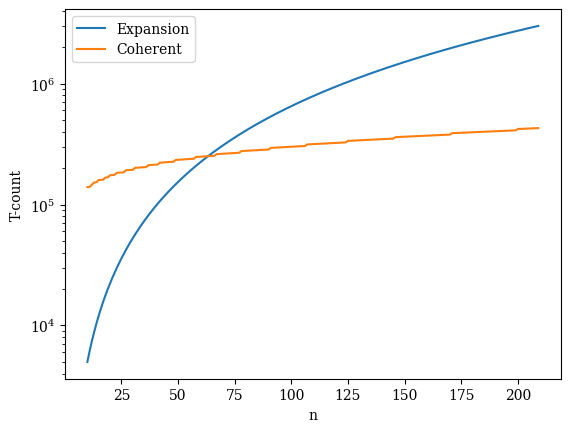
\includegraphics{Tcount.png}
    \caption{Approximate $T$-counts for the expansion and coherent methods of $U_A^{(r)}$ using $\epsilon = 10^{-6}$, $\Delta t = 0.01 \frac{1}{E_h}$, and $|\lambda_r|Y_r^2 = n\log_2{n} E_h$ estimated for hydrogen chain Hamiltonians.}
    \label{fig: Tcounts}
\end{figure}

%When is O(n log n) really better than n^2/2?

%Mention that if it's really diagonal, then we can just qdrift the rotations.

\section{Discussion}

The asymptotic (in $n$) advantage of the coherent method ($O(n\log_2{n})$) over the expansion method ($O(n^2\log_2{n})$) is only useful in $U_A^{(r)}$ if the number of $T$ gates in $U_R(u^{(r)})$ can also be reduced from $O(n^2\log_2(\frac{n}{\epsilon}))$. Otherwise, the latter asymptotically dominates and maintains the overall complexity unchanged.

In Chapter 3, we explore Hamiltonians for which it is the case that $U_R(u^{(r)})$ can be decomposed ``easily'' as such.


%%%%%%%%%%%%%%%% end table %%%%%%%%%%%%%%%%%%% 

